\documentclass[a4paper, 12pt]{article}
%\documentclass{book}

% Important Packages:
 \usepackage{amsmath}    % need for subequations
 \usepackage{amsfonts}
 \usepackage{amsthm}
 \usepackage{graphicx}   % need for figures
 \usepackage{verbatim}   % useful for program listings
 %\usepackage{subfig}  % use for side-by-side figures
 %\usepackage{wrapfig}
 %\usepackage{listings}	 % creates code blocks
 %\usepackage[colorlinks=true]{hyperref}   % use for hypertext links, including
                     % those to external documents and URLs
 %\usepackage{multirow}
 %\usepackage{tikz}
 %\usepackage{enumerate}
 %\usetikzlibrary{decorations.pathreplacing,decorations.pathmorphing}
 %\usetikzlibrary{calc}
 %\usepackage[colorinlistoftodos]{todonotes}
 \usepackage{tikz,tkz-euclide}
 
 \usetikzlibrary{calc,patterns,angles,quotes}
\usetkzobj{all}

\def\deg{^{\circ}}
\newcommand\heading[1]{\ \\\large{\textbf{#1}}}
\newcommand\ora[1]{\overrightarrow{#1}}

%------------------end---preamble--------------------
 
 % Useful macros 
 \def\tcb#1{\color{blue}{#1}}
 \def\tcr#1{\color{red}{#1}}	
 \def\tcg#1{\color{green}{#1}}
 \def\be{\begin{eqnarray}}	 	\def\ee{\end{eqnarray}}
 \def\bea{\begin{eqnarray}}	 	\def\eea{\end{eqnarray}}
 \def\bean{\begin{eqnarray*}}	\def\eean{\end{eqnarray*}}
 
 \def\D{\displaystyle}
 \def\T{\textstyle}
 \def\l{\left}
 \def\r{\right}
 \def\nf{n_{\!f}} % quark flavours
 \def\pa{\partial}
 \def\eg{e.\,g.}
 \def\ie{i.\,e.}

 \def\be{\begin{equation}}
 \def\ee{\end{equation}}
 \def\bea{\begin{eqnarray}}
 \def\eea{\end{eqnarray}}
 \def\bean{\begin{eqnarray*}}
 \def\eean{\end{eqnarray*}}
 \def\gsim{\mathrel{\rlap{\lower0.2em\hbox{$\sim$}}\raise0.2em\hbox{$>$}}}
 \def\ksim{\mathrel{\rlap{\lower0.2em\hbox{$\sim$}}\raise0.2em\hbox{$<$}}}
 \def\kg{\mathrel{\rlap{\lower0.25em\hbox{$>$}}\raise0.25em\hbox{$<$}}}
 
 \def\AA{${\buildrel_{\circ} \over {\mathrm{A}}}$}
 \def\bm#1{\mbox{\boldmath$#1$}}
 \newcommand{\eq}[1]{(\ref{#1})} 
 \def\pd{\partial}
 \def\d{\textrm{d}} 
 \def\T{\textstyle}
 \def\eg{e.\,g.}	% exempli gratia (for the sake of example)
 \def\ie{i.\,e.}	% id est (that is)


 % Page configuration:
 \topmargin -2.0cm
 \oddsidemargin -0.85cm
 \evensidemargin -0.85cm
 \textwidth 18cm
 \textheight 24cm
 
\begin{document}
\begin{center}
\textbf{Stellenbosch Camp December 2018 \\ Senior Test 2} \\
\textbf{Solutions}
\end{center}
\vspace{5mm}

\begin{enumerate}
    % EGMO 2013 solutions: https://www.egmo.org/egmos/egmo2/solutions.pdf

    % QUESTION 1
    \item[1.]   Taking the 1 over and factoring, we obtain $(n-1)(n+1) = 5 \cdot 2^m$. Note that $n$ is odd, which implies both $n-1$ and $n+1$ are even. Furthermore, gcd($n-1, n+1$) = 2. Therefore, we have either $v_2(n-1) = 1$ or $v_2(n+1) = 1$. Noting the cases for 5, we also have $v_5(n-1) = 1$ or $v_5(n+1) = 1$. This therefore yields the following possibilities:
\begin{align*}
    n - 1 &= 2 \quad \textrm{ or } \quad n - 1 = 2 \cdot 5 = 10 \\
    \textrm{ or } \quad  n + 1 &= 2 \quad \textrm{ or } \quad n + 1 = 2 \cdot 5 = 10 
\end{align*}
Noting all cases, one obtains that only $n=9$ yields a valid solution where $m = 4$. Thus the only solution is $(n, m) = (9, 4)$. \qed \\
    \vspace{5mm}
    
    % QUESTION 2
    \item[2.]  Let $[a_1, b_1]$ be the segment with the smallest right endpoint. If more than 7 segments contain $b_1$, then we are finished. If this number is $\leq 7$, then at least 43 segments lie completely to the right of $b_1$. From these segments, select $[a_2, b_2]$ with the smallest right endpoint. Then either $b_2$ belongs to 8 segments, or there exist 36 segments to the right of $b_2$.
    
    Continuing in this way, either we find a point belonging to eight segments, or we find seven pairwise disjoint segments $[a_1, b_1], [a_2, b_2], \dots, [a_7, b_7]$ such that to the right of $[a_k, b_k]$ lie at least $(50-7k)$ segments, i.e. to the right of $[a_7, b_7]$ lies at least one segment $[a_8, b_8]$.     \qed \\
    \vspace{5mm}
    
    % QUESTION 3
    \item[3.] Checking the first few cases, we find $a_2 = 2^2, a_3 = 5^2, a_4 = 13^2$, squares of every other term of the Fibonacci sequence defined by the equalities $F_1 = F_2 = 1$ and $F_{n+1} = F_n + F_{n-1}$ for $n \geq 2$. This suggests that $a_n = F_{2n-1}^2$ for all $n \geq 1$, which we will prove by induction.
    
    The claim is true for $n = 1, 2, 3, 4$. Assuming $a_k = F_{2k-1}^2$ for $k \leq n$, and subtracting $a_n = 7a_{n-1} - a_{n-2} - 2$ from $a_{n+1} = 7a_n - a_{n-1} - 2$, we obtain
    \begin{align*}
        a_{n+1} &= 8 a_n - 8 a_{n-1} + a_{n-2} \\
        &= 8 F_{2n-1}^2 - 8 F_{2n-3}^2 + F_{2n-5}^2
    \end{align*}
    It is not difficult to check that $F_{m-2} = 3 F_m - F_{m+2}$ for all $m \geq 2$. Thus, replacing $F_{2n-5}$ by $3 F_{2n-3} - F_{2n-1}$ yields
    \begin{align*}
        a_{n+1} &= 8 F_{2n-1}^2 - 8 F_{2n-3}^2 + (3 F_{2n-3} - F_{2n-1})^2 \\
        &= (3 F_{2n-1} - F_{2n-3} )^2 \\
        &= F_{2n+1}^2 .
    \end{align*}
    This therefore completes the proof by induction. \qed
    
    
    \newpage
    % QUESTION 4
    \item[4.]  
		
	First construct point $F$ as the intersection of $\Gamma$ and $BD$. Let $T$ be a point on the tangent of $\Gamma$ at $D$, such that $\angle BDT$ is acute.\\

	Using the fact that $TD$ is tangent to $\Gamma$ and the circumcircle of $ABD$.
	\begin{flalign}
		\angle FED=\angle BDT=\angle BAD \nonumber
	\end{flalign}

	So $AB||EF$. \marginnote{(1)} \\

	Using power of a point,the fact that $AC$ is tangent to $\Gamma$, and that $AC=AB$.
	\begin{flalign}
		AB^2=AC^2=DA \cdot AE \nonumber
	\end{flalign}

	So $AB$ is tangent to the circumcircle of $EBD$. \marginnote{(2)} \\

	Now, combining (1) and (2):
	\begin{flalign}
		\angle BEF=\angle EBA=\angle EDB=\angle EDF\nonumber
	\end{flalign}
	
	Thus, since $\angle BEF=\angle EDB \nonumber$, we have $BE$ is tangent to $\Gamma$, by the converse of Tan-Chord Th\textsuperscript{\underline{m}}.
	 \qed \\
	 \vspace{10mm}
	 
	 
	\begin{figure}[h!]
	\begin{center}
	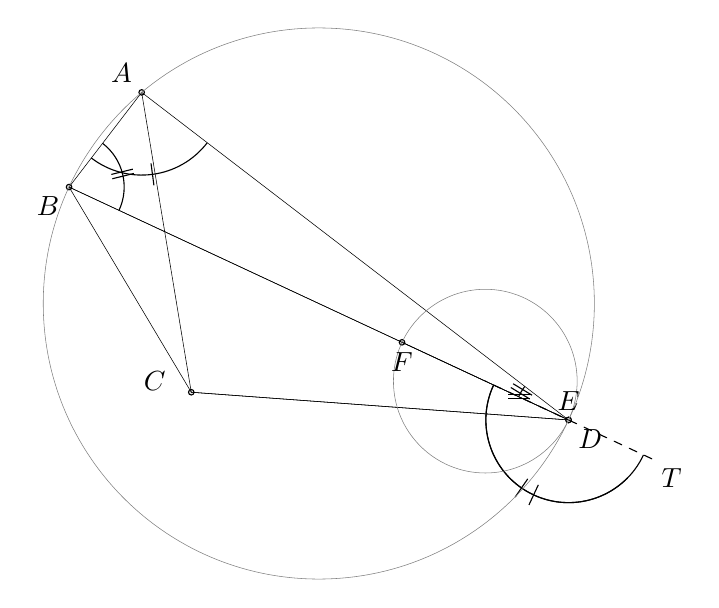
\begin{tikzpicture}[scale=3.5]
		% \useasboundingbox (-2,-2) rectangle  (2,2);
		\tkzDefPoint(0,0){O}
		\tkzDefPoint[label=120:$A$](130:1){A}
		\tkzDefPoint[label=-60:$D$](-25:1){D}
		\tkzDefBarycentricPoint(D=2,O=1) \tkzGetPoint{I}
		\tkzInterLC(D,A)(I,D)\tkzGetFirstPoint{E}
		\tkzTangent[at=E](I)\tkzGetPoint{t}
		\tkzInterLC(E,t)(O,A)\tkzGetSecondPoint{B}
		\tkzInterCC(A,B)(I,D)\tkzGetSecondPoint{C}
		\tkzInterLC(D,B)(I,D)\tkzGetSecondPoint{F}
		\tkzTangent[at=D](O)\tkzGetPoint{s}
		\tkzDefPointsBy[symmetry=center D](s){s1}
		\tkzMarkAngles[size=0.3,mark=|](B,A,D F,E,D B,D,s1)
		\tkzMarkAngles[size=0.2,mark=||](E,B,A B,E,F A,D,F)
		\tkzLabelPoint[below right](s1){$T$}
		\tkzDrawPoints(A,B,C,D,E,F)
		\tkzDrawSegments(A,B A,C A,E B,C B,E B,F C,D C,E D,E D,F E,F)
		\tkzDrawCircle(O,A)
		\tkzDrawCircle(I,D)
		\tkzLabelPoints[above](E)
		\tkzLabelPoints[below left](B)
		\tkzLabelPoints[below](F)
		\tkzLabelPoints[above left=-0.1 and 0.2](C)
		\tkzDrawLine[thin,dashed,add=1 and 0](D,s)
		\end{tikzpicture}
	\end{center}		
	\end{figure}
	 
	 
    \vspace{5mm}
    
    % QUESTION 5
    \item[5.]  Letting $x = y = 0$ yields $2f(0) = 4f(0)$, so $f(0) = 0$. We will prove by induction that $f(nz) = n^2f(z)$ for any positive integer $n$ and any rational number $z$.
    
    The claim holds for $n = 0$ and $n = 1$. Let $n \geq 2$ and suppose the claim holds for $n-1$ and $n-2$. Then letting $x = (n-1)z$ and $y = z$ in the given equation, we obtain
    \begin{align*}
        f(nz) + f((n-2)z) &= f((n-1)z + z) + f((n-1)z - z) \\
        &= 2f((n-1)z) + 2f(z)
    \end{align*}
    thus
    \begin{align*}
        f(nz) &= 2f((n-1)z) + 2f(z) - f((n-2)z) \\
        &= 2(n-1)^2 f(z) + 2f(z) - (n-2)^2 f(z) \\
        &= (2n^2 - 4n + 2 + 2 - n^2 + 4n - 4) f(z) \\
        &= n^2 f(z)
    \end{align*}
    and the claim holds by induction.
    
    Letting $x = 0$ in the given equation gives
    \begin{equation*}
        f(y) + f(-y) = 2f(0) + 2f(y) = 2f(y)
    \end{equation*}
    so $f(-y) = f(y)$ for all rational $y$; thus $f(nz) = n^2 f(z)$ for all integers $n$.
    
    Now let $k = f(1)$; then for any rational number $x = p/q$,
    \begin{equation*}
        q^2 f(x) = f(qx) = f(p) = p^2 f(1) = kp^2
    \end{equation*}
    thus
    \begin{equation*}
        f(x) = kp^2/q^2 = kx^2 .
    \end{equation*}
    
    We therefore obtain $f(x) = kx^2$ where $k \in \mathbb{Q}$. One can easily check that these solutions satisfy the given functional equation.    \qed

    

\end{enumerate}
\end{document}




